\documentclass{article}
\usepackage[utf8]{inputenc}
\usepackage{attachfile2}
\usepackage{hyperref}
\usepackage{booktabs}
\usepackage{graphicx}
\usepackage{subcaption}
\usepackage{float}
\usepackage{amssymb}
\usepackage{amsfonts}
\usepackage{amsmath}
\usepackage{bookmark}
\usepackage{listings}
\lstset{
  basicstyle=\ttfamily\small,
  numbers=left, 
  numberstyle=\tiny,
  frame=single,
  captionpos=b
}

\newcommand{\IP}{../results}

\title{\textbf{Network robustness} \\ \vspace{0.5em}
  \large Network Analysis - Assignment 3}
\author{Enrico Pezzano}
\date{June 2025}

\begin{document}
\maketitle

\section{Introduction}
In this assignment, I will analyze how the structure of a network affects its resilience to node failures or targeted attacks.
I first implemented and compared four attack strategies (random failures, highest-degree removal, PageRank-based and betweenness-based removals) on small toy graphs (\S\ref{sec:toy}) and then on the same political-blogs network (\S\ref{sec:polblogs}) of the previous two assignments.
After that, I tried to improve the robustness of each of the mentioned networks by adding edges in “rings” among the neighbours of the top-$k$ highest-degree nodes (\S\ref{sec:building}).

Additionally, since the \texttt{polblogs} network did not show interesting results, I searched for the community (subgraph) with the lowest theoretical percolation threshold $f_c$ and repeated the experiments on that worst component (\S\ref{sec:worst_community}), trying to improve its robustness as well, but the results were not as expected.


\section{Methodology}\label{sec:met}
First of all, I implemented the attack strategies as $4$ different functions, each of which takes a graph, a fraction of nodes to remove, and a number of steps that simply corresponds to the number of iterations to perform, removing the specified fraction of nodes at each step.
Note that a higher number of steps means that the attack simulation will be more detailed, but the execution time will also increase.
The four attack strategies are, as showed in the AulaWeb example, random failures, highest-degree removal, PageRank-based and betweenness-based removals.

After the attacks are executed, I tried to improve the robustness of the network by adding edges in “rings” among the neighbours of the top-$k$ highest-degree nodes and also including a \emph{randomized} version of the original graph with the same degree sequence, generated via double-edge swaps, in order to use it as a baseline for comparison.
The following listing shows the python code for what I have just described.

\begin{lstlisting}[language=Python, caption={Attack strategies.}]
def attack_random(G, rm_fraction=0.01, steps=100):
    nodes = list(G.nodes())
    random.shuffle(nodes)
    batch_size = max(1, int(rm_fraction * len(nodes)))
    sizes, Gc = [], G.copy()
    for i in range(steps):
        rem = nodes[i*batch_size:(i+1)*batch_size]
        if not rem:
            break
        Gc.remove_nodes_from(rem)
        sizes.append(giant_component_size(Gc))
    return sizes

def attack_highest_degree(G,rm_fraction=0.01,steps=100):
    Gc, sizes = G.copy(), []
    batch_size = max(1, int(rm_fraction * len(G)))
    for _ in range(steps):
        to_rm = [n for n,_ in sorted(Gc.degree(),
                                         key=lambda x: x[1],
                                         reverse=True)
                                         [:batch_size]]
        if not to_rm: break
        Gc.remove_nodes_from(to_rm)
        sizes.append(giant_component_size(Gc))
    return sizes

def attack_pagerank(G, rm_fraction=0.01, steps=100):
  Gc, sizes = G.copy(), []
  batch_size = max(1, int(rm_fraction * len(G)))
  for _ in range(steps):
    to_rm = [n for n,_ in sorted(nx.pagerank(Gc).items(),
                                 key=lambda x: x[1],
                                 reverse=True)[:batch_size]]
        if not to_rm: break
        Gc.remove_nodes_from(to_rm)
        sizes.append(giant_component_size(Gc))
    return sizes

def attack_betweenness(G, rm_fraction=0.01, steps=100):
    Gc, sizes = G.copy(), []
    batch_size = max(1, int(rm_fraction * len(G)))
    for _ in range(steps):
        to_rm = [n for n,_ in sorted(
         nx.betweenness_centrality(Gc).items(),
                                 key=lambda x: x[1],
                                 reverse=True)[:batch_size]]
        if not to_rm: break
        Gc.remove_nodes_from(to_rm)
        sizes.append(giant_component_size(Gc))
    return sizes


results_real = {
    'random':
        attack_random(G, rm_fraction=0.01, steps=100),
    'degree':
        attack_highest_degree(G,rm_fraction=0.01,steps=100),
    'pagerank':
        attack_pagerank(G, rm_fraction=0.01, steps=100),
    'betweenness':
        attack_betweenness(G, rm_fraction=0.01, steps=100),
}
\end{lstlisting}

\begin{lstlisting}[language=Python, caption={Edge augmentation.}]
def add_ring_among_high_degree(G, top_k=3):
    Gc = G.copy()
    top_nodes = sorted(Gc.degree(), 
                       key=lambda x: x[1], 
                       reverse=True
                      )[:top_k]
    for n, _ in top_nodes:
        neigh = list(Gc.neighbors(n))
        if len(neigh) > 2:
            for i in range(len(neigh)):
                u, v = neigh[i], neigh[(i+1) % len(neigh)]
                if not Gc.has_edge(u, v):
                    Gc.add_edge(u, v)
    return Gc

def randomize_graph(G, n_swaps=None):
    Gc = G.copy()
    if n_swaps is None:
        n_swaps = Gc.number_of_edges() * 10
    nx.double_edge_swap(Gc, n_swaps, max_tries=n_swaps * 10)
    return Gc


G_rand  = randomize_graph(G)
G_ring1 = add_ring_among_high_degree(G, top_k=3)
G_ring2 = add_ring_among_high_degree(G_ring1,  top_k=3)
G_ring3 = add_ring_among_high_degree(G_ring2,  top_k=3)
\end{lstlisting}

Finally, I computed the theoretical critical threshold $f_c$ for each graph, using the formula 
$$
f_c \;=\;1 \;-\;\frac{1}{\frac{\langle k^2\rangle}{\langle k\rangle}-1}\,.
$$

and the first and second moments of the degree distribution using the following python code.
\begin{lstlisting}[language=Python, caption={First and second moments of the degree distribution.}]
degs = np.array([d for _, d in Gs.degree()])
k1, k2 = degs.mean(), (degs**2).mean()
\end{lstlisting}

I then printed the results in a table and plotted the giant component size during the attacks, as seen in the example in AulaWeb.

Additionally, I used the \texttt{greedy\_modularity\_communities} function from \texttt{NetworkX}, i.e. Clauset-Newman-Moore algorithm, to detect communities in the graph and identify the one with the lowest valid $f_c$ (and at least 10 nodes), which I then used to repeat the robustness experiments on that worst component.


\section{Toy Graph}\label{sec:toy}
I first tested my code on a small undirected graph of 100 nodes, using the \texttt{NetworkX} functions for synthetic networks, in particular, I choose the Barabási-Albert and the Erdos-Rényi models. 
The following figures \ref{fig:toy:attacks} show the results of the various attacks.

\begin{figure}[H]
   \centering
   \begin{subfigure}{0.49\textwidth}
      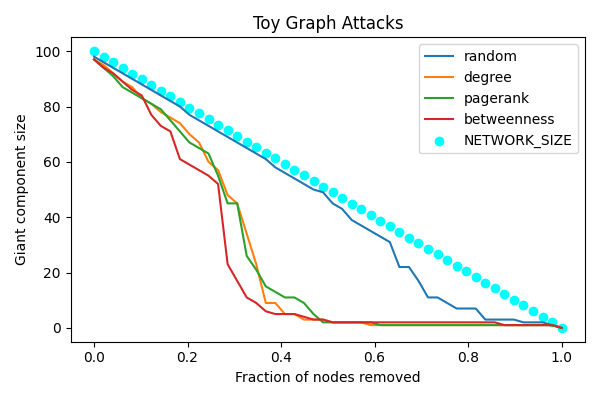
\includegraphics[width=\linewidth]{\IP/ba_toy_graph_attacks.png}
      \caption{Barabási-Albert graph (N=100)}
      \label{fig:toy:ba}
   \end{subfigure}
   \hfill
   \begin{subfigure}{0.49\textwidth}
      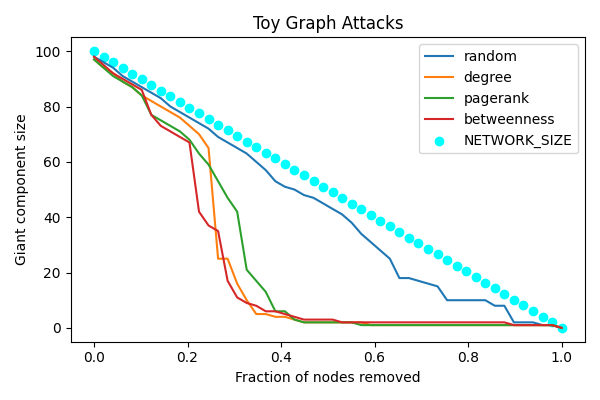
\includegraphics[width=\linewidth]{\IP/toy_graph_attacks.png}
      \caption{Erdős-Rényi graph (N=100)}
      \label{fig:toy:er}
   \end{subfigure}
   \caption{Attack strategies on toy graphs: giant component size vs. fraction of nodes removed.}
   \label{fig:toy:attacks}
\end{figure}

The Barabási-Albert graph is slightly more robust than the Erdős-Rényi graph to degree and PageRank attacks, but both graphs are very fragile to betweenness attacks, which break the giant component very quickly.
Random failures are the least destructive, as expected.


\section{PolBlogs Graph}\label{sec:polblogs}
The successive part of the assignment was to apply the same attack strategies to the chosen network: in my case, I used the usual \texttt{polblogs} network, but this time I removed immediately the two isolated nodes, in order to convert it into an undirected graph with $N=1222$ nodes and $L=16714$ edges, which of course is the largest connected component of the original directed graph.

Successively, I applied the four attack strategies to this network, as described in the previous section, and plotted the giant component size as a function of the fraction of nodes removed.
Figure \ref{fig:polblogs_attacks} shows the results of the attacks on the \texttt{polblogs} network, with its original robustness. 

\begin{figure}[H]
  \centering
  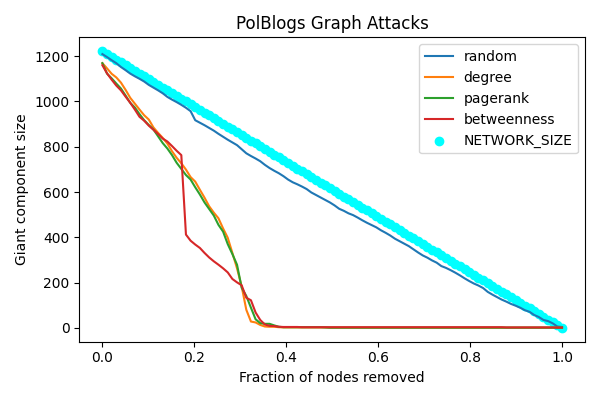
\includegraphics[width=1\textwidth]{\IP/polblogs_graph_attacks.png}
  \caption{PolBlogs: giant-component size under different attack strategies.}
  \label{fig:polblogs_attacks}
\end{figure}

The results are very similar with the toy experiments: random failures cause progressive degradation in the network performance, but with little to no effect on the giant component size, which remains almost constant until the end of the attack.
On the other hand, attacks on the highest degree nodes, PageRank, and betweenness severely damage the graph structure, with the betweenness attack being the most harmful, but not by a big margin.

\section{Building robustness}\label{sec:building}
As requested by the assignment, I tried to improve the robustness of the chosen network by adding edges in “rings” among the neighbours of the top-$k$ highest-degree nodes, and I hardcoded $k=40, 80, 120$, since they were only 3 iterations.
I wanted to replicate the example on AulaWeb, where there was 3 iterations of adding one ring at a time on a $35$ nodes network; so, for my $1222$ nodes network, I decided to go for the $10\%$ of the nodes, which is $122$ nodes, and I added $40$ rings at a time, for a total of $3$ iterations.

I used the \texttt{python} code mentioned in the methodology section \ref{sec:met} to add the said rings, and then computed the first and second moments of the degree distribution, as well as the critical threshold $f_c$ before and after the edge additions.

The following table summarizes the results of the robustness improvement on the chosen network.

\begin{table}[H]
  \centering
  \caption{PolBlogs robustness improvement.}\label{tab:polblogs:improv}
  \begin{tabular}{lcccc}
    \toprule
    Graph & Size (N,L) & $\langle k\rangle$ & $\langle k^2\rangle$ & $f_c$ \\
    \midrule
    Original         & N=1222, L=16714 & 27.36 & 2222.98 & 0.9875 \\
    Randomized       & N=1222, L=16714 & 27.36 & 2222.98 & 0.9875 \\
    After 40 rings   & N=1222, L=20174 & 33.02 & 2755.23 & 0.9879 \\
    After 80 rings   & N=1222, L=21282 & 34.83 & 2959.87 & 0.9881 \\
    After 120 rings  & N=1222, L=23713 & 38.81 & 3441.95 & 0.9886 \\
    \bottomrule
  \end{tabular}
   \label{tab:polblogs:summary}
\end{table}

We can see that both the mean degree $\langle k\rangle$ and the second moment $\langle k^2\rangle$ increase after each ring addition, which is expected since we are adding edges.
% 
% In short: your PolBlogs graph has such a large variance in degrees (thanks to its hub‐and‐spoke structure) that its random‐failure threshold 
% 𝑓
% 𝑐
% f 
% c
% ​
%   sits very close to 1. That’s exactly what the theory predicts for a network with a heavy‐tailed degree distribution.
% 
The critical threshold $f_c$ also increases, but only slightly, which is not surprising since the \texttt{polblogs} network is already quite robust, with a high inital $f_c$ value of $0.9875$, due of its large variance in the degree distribution, which is a consequence of its hub-and-spoke structure, reflecting the underlying political blogosphere.
Nonetheless, the edge additions do improve the robustness of the network, as we can see from the increasing $f_c$ values after each iteration.

\paragraph{Resultant Plots}
The following figure \ref{fig:polblogs_randomized} shows the results of the same 4 types of attacks mentioned before, but on the randomized version of the \texttt{polblogs} network, which has the same degree sequence as the original graph, but with edges randomly shuffled.

\begin{figure}[H]
  \centering
  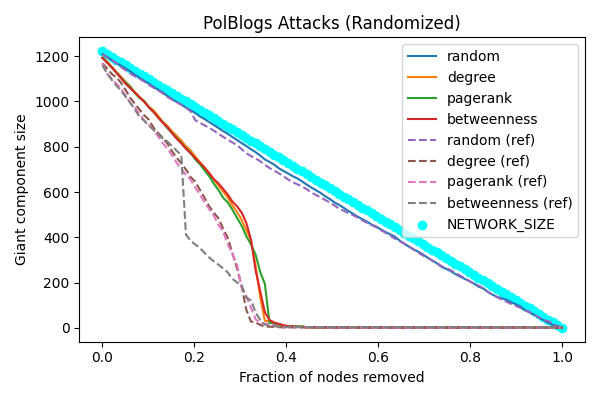
\includegraphics[width=1\textwidth]{\IP/polblogs_attacks_(randomized).png}
  \caption{PolBlogs: giant-component size under different attack strategies on the randomized graph.}
  \label{fig:polblogs_randomized}
\end{figure}

The randomized graph shows a similar behaviour to the original one, but with smoother curves, as expected.
The giant component size decreases linearly with the fraction of nodes removed under the random failures attack, while the targeted attacks cause a more abrupt drop in the giant component size, after around $38\%$ of nodes removed. This graph proved to be slightly more resilient to the betweenness attack, compared to the original \texttt{polblogs} graph.

The folloing figures, instead \ref{fig:polblogs_ring1}, \ref{fig:polblogs_ring2} and \ref{fig:polblogs_ring3}, show the results of the same attacks on the graph after each ring addition, i.e. after adding $40$, $80$ and $120$ rings, respectively.

\begin{figure}[H]
  \centering
  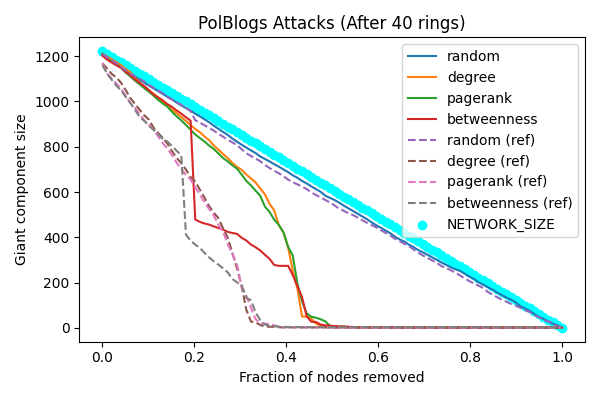
\includegraphics[width=1\textwidth]{\IP/polblogs_attacks_(after_40_rings).png}
  \caption{PolBlogs: giant-component size under different attack strategies after adding 40 rings.}
  \label{fig:polblogs_ring1}
\end{figure}
\begin{figure}[H]
  \centering
  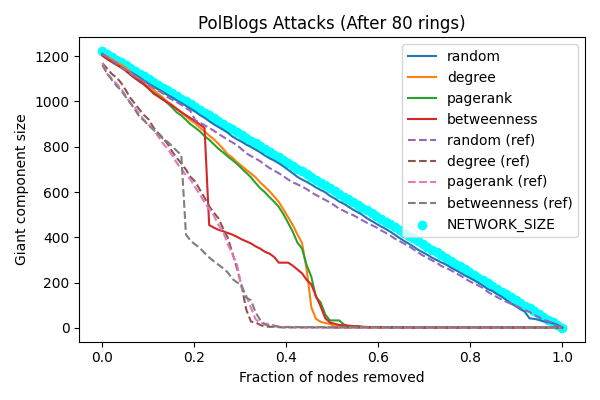
\includegraphics[width=1\textwidth]{\IP/polblogs_attacks_(after_80_rings).png}
  \caption{PolBlogs: giant-component size under different attack strategies after adding 80 rings.}
  \label{fig:polblogs_ring2}
\end{figure}
\begin{figure}[H]
  \centering
  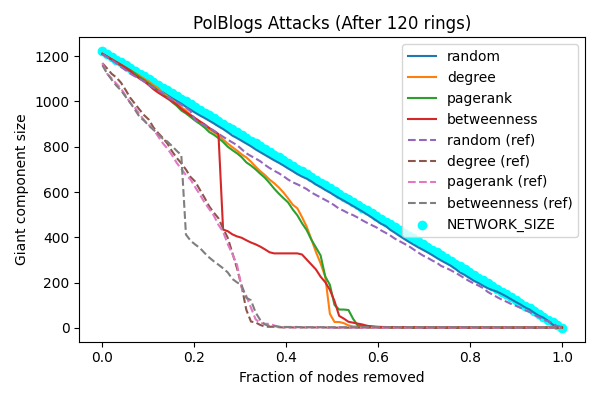
\includegraphics[width=1\textwidth]{\IP/polblogs_attacks_(after_120_rings).png}
  \caption{PolBlogs: giant-component size under different attack strategies after adding 120 rings.}
  \label{fig:polblogs_ring3}
\end{figure}

Sadly, due to the critical threshold $f_c$ increasing only slightly, the robustness improvement betweennes the modified graphs is difficult to observe by the naked eye.
Nonetheless, we can computed $f_c$ for each of the graphs after the ring additions, and have mathematical proof of said improvement, as shown in Table \ref{tab:polblogs:summary}.

Instead, we can observe the differences between the original plot of the \texttt(polblogs) network under attack, versus the last improved graph with 120 rings added and $f_c=0.9886$ versus $f_c=0.9875$. In particular, the random failures attack is slightly less destructive, the degree attack and the PageRank attack make the giant component size drop more gradually and around $50\%$ of nodes removed instead of the original $38\%$, and the betweenness attack is still the most destructive, but this time with a less abrupt drop in the giant component size, falling around $25\%$ of nodes removed instead of the original $18\%$, completely falling at around $57\%$ of nodes removed instead of the original $38\%$.


\section{Community with the worst critical threshold}\label{sec:worst_community}
Since the \texttt{polblogs} network did not show interesting results, only a $f_c$ improvement of $0.0011$ was observed after adding $120$ rings on $1222$ nodes, I thought that it would be interesting to search for the community with the lowest critical threshold $f_c$ and repeat the robustness experiments on that worst component, in order to see if the edge additions would have a more significant effect on the robustness of the network, even thought it does not make any sense from a theoretical point of view, since the critical threshold $f_c$ is defined for networks with $N\to\infty$, but still, I wanted to try it.

I used the \texttt{NetworkX} function \texttt{greedy\_modularity\_communities}, i.e. the Clauset Newman Moore algorithm, to detect communities with at least 10 nodes. The following listing \ref{lst:worst_community} shows what already described, and the Table \ref{tab:comms:fc} lists the detected communities and their relative $f_c$ values.

\begin{lstlisting}[language=Python, caption={Finding the worst community.}, label={lst:worst_community}]
comms = community.greedy_modularity_communities(G_real)
print(f"\nDetected {len(comms)} communities")
for i, nodes in enumerate(comms):
    sub = G_real.subgraph(nodes)
    degs = np.array([d for _,d in sub.degree()])
    k1, k2 = degs.mean(), (degs**2).mean()
    denom = k2/k1 - 1 if k1>0 else -1
    fc = (1 - 1/denom) if denom>0 else float('nan')
    print(f"\tCommunity {i}: N={sub.number_of_nodes()}, 
                             L={sub.number_of_edges()}, 
                             f_c={fc:.4f}")

MIN_SIZE = 10
cands = []
for i, nodes in enumerate(comms):
    if len(nodes) < MIN_SIZE: continue
    sub = G_real.subgraph(nodes).copy()
    degs = np.array([d for _,d in sub.degree()])
    k1, k2 = degs.mean(), (degs**2).mean()
    denom = k2/k1 - 1 if k1>0 else -1
    if denom<=0: continue
    fc = 1 - 1/denom
    cands.append((f"Community {i}", sub, fc))

if not cands:
    print("No valid community >= MIN_SIZE with fc>0.")
    exit()

worst_name, worst_subG, worst_fc = min(
                                       cands, 
                                       key=lambda x: x[2]
                                      )
Nw, Lw = worst_subG.number_of_nodes(), 
         worst_subG.number_of_edges()
\end{lstlisting}

\begin{table}[H]
  \centering
  \caption{Detected communities and their $f_c$.}\label{tab:comms:fc}
  \begin{tabular}{lcc}
    \toprule
    Community & Size (N,L) & $f_c$ \\
    \midrule
      0 & 634, 8163  & 0.9858 \\
      1 & 544, 7226  & 0.9868 \\
      2 & 23, 22     & 0.8736 \\
      3 & 5, 5       & 0.2857 \\
      4 & 4, 3       & 0.0000 \\
      5 & 3, 2       & -1.0000 \\
      6 & 3, 2       & -1.0000 \\
      7 & 2, 1       & nan \\
      8 & 2, 1       & nan \\
      9 & 2, 1       & nan \\
  \end{tabular}
\end{table}

The community with the lowest $f_c$ is Community $2$, which has only $23$ nodes and $22$ edges, with a critical threshold of $0.8736$, lower than the other communities, and lower than the original \texttt{polblogs} network. Additionally, the chosen community is one out of three with at least $10$ nodes, which is the minimum size that I considered valid for a community, since smaller communities are not very interesting for this kind of analysis. Then, I computed the first and second moments of the degree distribution for this community, and I obtained $\langle k\rangle=1.91$ and $\langle k^2\rangle=17.04$, which resulterd in the critical threshold $f_c=0.8736$.

Successively, I repeated the four attack simulations on this worst subgraph (Community 2), and the results are summarized in the following Figure \ref{fig:bonus_attacks}.

\begin{figure}[H]
  \centering
  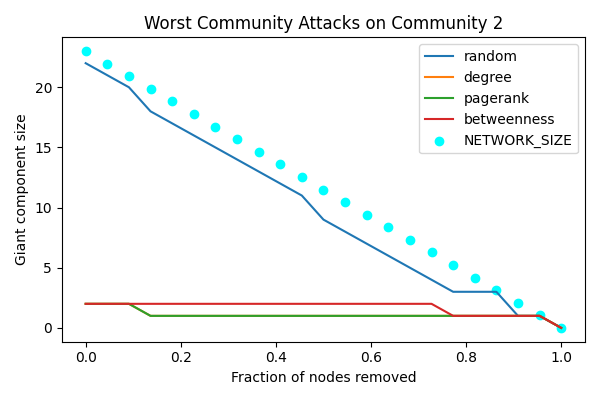
\includegraphics[width=1\textwidth]{\IP/worst_community_attacks_on_community_2.png}
  \caption{Community 2: giant-component size under different attack strategies.}
  \label{fig:bonus_attacks}
\end{figure}

The resultant graph show, this time, shows a very different behaviour compared to the \texttt{polblogs} network: the random failures attack causes a very quick degradation of the giant component size, which drops to zero after removing only $10\%$ of the nodes, while the targeted attacks are still much more destructive. This shows that even if the critical threshold $f_c$ is not very low, the community is very fragile to failures, which is a common characteristic of small communities.

As done for the \texttt{polblogs} network, I tried to improve the robustness of this community by adding edges in “rings” among the neighbours of the top-$k$ highest-degree nodes, and I hardcoded $k=3$, since this time the community is very small, with only $N=23$ nodes, so I decided to add one ring at a time, for a total of $3$ iterations, for the top $3$ highest-degree nodes. The following Table \ref{tab:bonus:improv} summarizes the results.

\begin{table}[H]
  \centering
  \caption{Robustness improvement on the worst community.}\label{tab:bonus:improv}
  \begin{tabular}{lcccc}
    \toprule
    Graph           & Size (N,L) & $\langle k\rangle$ & $\langle k^2\rangle$ & $f_c$ \\
    \midrule
    Original        & N=23, L=22 & 1.91 & 17.04 & 0.8736 \\
    Randomized      & N=23, L=22 & 1.91 & 17.04 & 0.8736 \\
    After 1 ring    & N=23, L=41 & 3.57 & 24.17 & 0.827  \\
    After 2 rings   & N=23, L=44 & 3.83 & 27.39 & 0.8376 \\
    After 3 rings   & N=23, L=49 & 4.26 & 32.35 & 0.8483 \\
    \bottomrule
  \end{tabular}
\end{table}

The results show that the mean degree $\langle k\rangle$ and the second moment $\langle k^2\rangle$ increase after each ring addition, as expected, but the critical threshold $f_c$ actually decreases after the first ring addition, which is not what I expected.

This behavior can be explained by the fact that adding edges in a small community like this one tends to make the degree distribution more homogeneous, thus reducing the ratio $\langle k^2\rangle/\langle k\rangle$ and consequently lowering $f_c$. This is in line with the findings from the percolation theory discussed in the Appendix \ref{sec:appendix}. The following Figure \ref{fig:bonus_ring1}, \ref{fig:bonus_ring2} and \ref{fig:bonus_ring3} show the results of the attacks on the community after each ring addition, i.e. after adding $1$, $2$ and $3$ rings, respectively.

\begin{figure}[H]
  \centering
  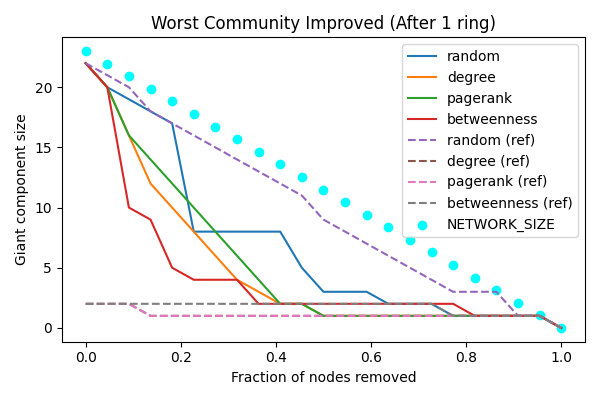
\includegraphics[width=1\textwidth]{\IP/worst_community_improved_(after_1_ring).png}
  \caption{Community 2: giant-component size under different attack strategies after adding 1 ring.}
  \label{fig:bonus_ring1}
\end{figure}
\begin{figure}[H]
   \centering
   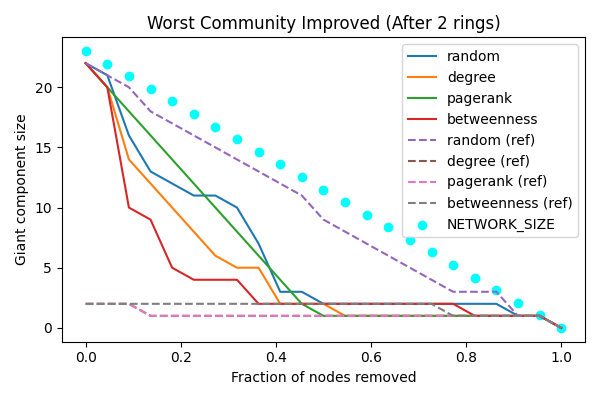
\includegraphics[width=1\textwidth]{\IP/worst_community_improved_(after_2_rings).png}
  \caption{Community 2: giant-component size under different attack strategies after adding 2 rings.}
  \label{fig:bonus_ring2}
\end{figure}
\begin{figure}[H]
  \centering
  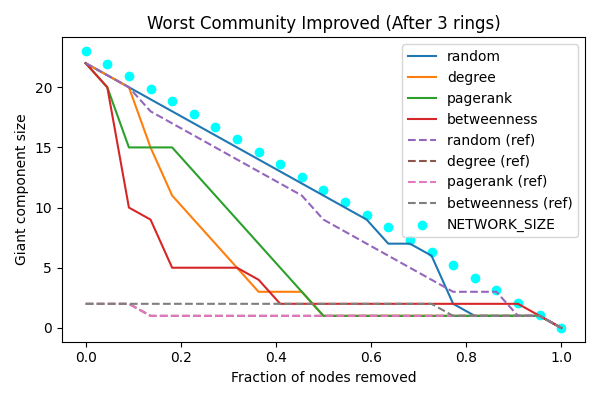
\includegraphics[width=1\textwidth]{\IP/worst_community_improved_(after_3_rings).png}
  \caption{Community 2: giant-component size under different attack strategies after adding 3 rings.}
  \label{fig:bonus_ring3}
\end{figure}

The final resultant plots show a very different community compared to the original \texttt{Community 2} graph: a more robust network, each time with more rings. In particular, the random failures attack is still the least destructive, followed by the remaining three targeted attacks.

It is the opposite of what I expected from the Table \ref{tab:bonus:improv}, where the critical threshold $f_c$ lowers after the first ring addition. 

The contrast between the various expectations and the actual results can be explained by the fact that the \texttt{Molloy-Reed} formula behind the critical threshold $f_c$ is based on the assumption that $N$ is in a very large limit, thus ignoring small or finite networks side-effects, and loops or clustering effects, which are more pronounced in small networks like \texttt{Community 2}.


\section{Conclusions}
In this assignment, I have explored the robustness of networks against node failures and targeted attacks, focusing on the effects of different attack strategies and edge additions to improve resilience.
I implemented four attack strategies (random failures, highest-degree removal, PageRank-based and betweenness-based removals) on both toy and real networks, specifically the \texttt{polblogs} network, and analyzed the giant component size as a function of the fraction of nodes removed.
I also attempted to improve the robustness of the networks by adding edges in “rings” among the neighbours of the top-$k$ highest-degree nodes, and I observed that this strategy can improve the robustness of the network, but only slightly, especially for the \texttt{polblogs} network.

In the end, I observed that targeted removals are far more destructive than random failures, and that the betweenness attack is the most harmful, followed by the highest-degree and PageRank attacks.

Additionally, I tried to isolate the weakest subgraph (Community 2) of the \texttt{polblogs} network, which had the lowest theoretical critical threshold $f_c$, and repeated the robustness experiments on that worst component, finding that the edge additions did not improve the robustness as expected, but rather decreased the critical threshold $f_c$ after the first ring addition, due to the small size of the community and the resulting homogeneity in the degree distribution.


\appendix \label{sec:appendix}

\section[Why fc can decrease under ring addition]{Why $f_c$ can decrease under ring addition}
The critical threshold $f_c$ is defined as the fraction of nodes that can be removed before the giant component disappears, and it is given by the formula
\[
  f_c \;=\;1\;-\;\frac{1}{\tfrac{\langle k^2\rangle}{\langle k\rangle}-1}.
\]
Although ring additions raise both $\langle k\rangle$ and $\langle k^2\rangle$, they can \emph{lower} the ratio $\langle k^2\rangle/\langle k\rangle$ if they preferentially boost mid-degree nodes, thus decreasing $f_c$.  Indeed, an alternative “spoke” strategy linking high-degree to low-degree nodes can increase variance more, pushing $f_c$ upward.

This happens because the ring addition strategy tends to make the degree distribution more homogeneous, i.e. ring-adding among neighbors of top-degree nodes tends to boost the degrees of mid or low-degree nodes more than it boosts the variance of the distribution, thus reducing the ratio $\langle k^2\rangle/\langle k\rangle$ and consequently, the degree distribution becomes more "flat", lowering $f_c$.


\section{Standard Output}
The following is the standard output of the code used in this assignment, which includes the results of the attack simulations, the robustness improvement after edge additions, and the critical threshold $f_c$ for each graph.

\attachfile{../results/results.txt}{Standard Output}


\end{document}